%% main.tex
%% Copyright Zhuowen Yuan
%
% This work may be distributed and/or modified under the
% conditions of the LaTeX Project Public License, either version 1.3
% of this license or (at your option) any later version.
% The latest version of this license is in
%   http://www.latex-project.org/lppl.txt
% and version 1.3 or later is part of all distributions of LaTeX
% version 2005/12/01 or later.
%
% This work has the LPPL maintenance status `maintained'.
% 
% The Current Maintainer of this work is Zhuowen Yuan.
%
% This work consists of the files main.tex and macro.tex.

\documentclass[a4paper,zihao=-4,UTF8]{ctexart}
\pagestyle{plain}
\date{}
\usepackage[top=1.0in, bottom=1.0in, left=1.25in, right=1.25in]{geometry} 
\setlength{\baselineskip}{20pt}
\usepackage{titlesec}
\usepackage{zhnumber}
\usepackage{abstract}
\usepackage{indentfirst}
\setlength{\parindent}{2em}
\usepackage{color}   % May be necessary if you want to color links
\usepackage{hyperref}
\hypersetup{
    colorlinks=true, %set true if you want colored links
    linktoc=all,     %set to all if you want both sections and subsections linked
    linkcolor=black,  %choose some color if you want links to stand out
}
\usepackage{fontspec}

% set font for English
\setmainfont{Times New Roman}
\setsansfont{Arial}
\setromanfont{Times New Roman}
% the following two are to support combined Chinese and English
\newcommand{\hei}[1]{\heiti\sffamily #1}
\newcommand{\song}[1]{\songti\rmfamily #1}


% setup style for table of contents
\usepackage{titlesec}
\usepackage{titletoc}
\usepackage{tocloft}
\titlecontents{section}[1em]{\zihao{-4}}{\contentslabel{1em}}{\hspace{-1em}}{\titlerule*[0.5pc]{$.$}\contentspage}
\titlecontents{subsection}[3em]{\zihao{-4}}{\contentslabel{2em}}{\hspace{-2em}}{\titlerule*[0.5pc]{$.$}\contentspage}
\titlecontents{subsubsection}[5em]{\zihao{-4}}{\contentslabel{3em}}{\hspace{-3em}}{\titlerule*[0.5pc]{$.$}\contentspage}
\renewcommand{\contentsname}{目~录 }
\usepackage{tocloft}
\renewcommand{\cfttoctitlefont}{\hfill\zihao{2}\heiti}
\renewcommand{\cftaftertoctitle}{\hfill}

% update references to Chinese style, font size and type can also be set here
\usepackage{caption}
% uncomment this if you want to use "第一章" instead of "第 1 章"
% \renewcommand\thesection{\zhnum{section}}
\titleformat{\section}{\centering\hei\zihao{-2}}{第~\thesection~章}{1em}{}[]
\titleformat{\subsection}{\hei\zihao{-3}}{\arabic{section}.\arabic{subsection}}{1em}{}[]
\titleformat{\subsubsection}{\hei\zihao{4}}{\arabic{section}.\arabic{subsection}.\arabic{subsubsection}}{1em}{}[]
\renewcommand{\abstractnamefont}{\hei\zihao{-2}}
\renewcommand{\abstracttextfont}{}
% \renewenvironment{abstract}{\begin{center}{\hei\zihao{-2}摘~要}\end{center}\par} \\
% \newenvironment{abstract-en}{\begin{center}{\hei\zihao{-2}Abstract}\end{center}\par}

\renewcommand{\figurename}{图}
\renewcommand{\tablename}{表}
\renewcommand{\thefigure} {\arabic{section}-\arabic{figure}}
\renewcommand{\theequation}{\arabic{section}.\arabic{equation}}
\renewcommand{\thetable} {\arabic{section}-\arabic{table}}
\captionsetup{labelsep=space} 


% title text
\newcommand{\mytitle}{yzw今天拖地了没}

% header
\usepackage{fancyhdr}
\pagestyle{fancy}
\fancyhead[L]{\kaishu\zihao{-5}\mytitle}
\fancyhead[R]{\kaishu\zihao{-5}\leftmark}
\renewcommand\headrulewidth{.5pt}
\renewcommand\footrulewidth{0pt}

% for hype-reference of "section*" to work properly
\usepackage{xparse}
\let\oldsection\section
\makeatletter
\newcounter{@secnumdepth}
\RenewDocumentCommand{\section}{s o m}{%
  \IfBooleanTF{#1}
    {\setcounter{@secnumdepth}{\value{secnumdepth}}% Store secnumdepth
     \setcounter{secnumdepth}{0}% Print only up to \chapter numbers
     \oldsection{#3}% \section*
     \setcounter{secnumdepth}{\value{@secnumdepth}}}% Restore secnumdepth
    {\IfValueTF{#2}% \section
       {\oldsection[#2]{#3}}% \section[.]{..}
       {\oldsection{#3}}}% \section{..}
}
\makeatother

% use GB/T 7714—2015 BibTeX Style
\usepackage{gbt7714}
\bibliographystyle{gbt7714-numerical}




% common packages
\usepackage{booktabs}
\usepackage{multirow}
\usepackage{graphicx}
\usepackage{enumitem}
\usepackage{amsmath,amssymb}
\usepackage{xcolor,colortbl}
\newcommand{\zw}[1]{\textcolor{cyan}{(Zhuowen: #1)}}
\usepackage[capitalize]{cleveref}  % Support for easy cross-referencing
\crefname{figure}{图}{图}
\crefname{table}{表}{表}
\crefname{equation}{公式}{公式}


\begin{document}
\title{\hei\zihao{-2}\mytitle}
\maketitle
\thispagestyle{empty}
\newpage


\pagenumbering{Roman}
\tableofcontents
\newpage


\pagenumbering{arabic}
\setcounter{page}{1}
\section*{摘~要}
本文提出了一种新型的加辣椒的番茄炒蛋烹饪法.其最重要的理念是要加辣椒.我们发现江苏的番茄炒蛋太甜,安徽的番茄炒蛋太咸,而本质上最好的解决方法就是加辣椒.从众多的辣椒中,我们从各种本性中进行分析,发现一个关键点是使用成熟度刚刚好的绿色的墨西哥辣椒.它由于个头小,不会喧宾夺主;由于绿色,增加了菜肴的颜色丰富度.最重要的是,这玩意真他娘的辣,谁吃谁知道.我们做了大量实验,发现老少咸宜,凡是吃了辣椒的都会快速吃完自己的米饭,可见这碗加辣椒的番茄炒蛋让人食欲大增.

% keywords
\vspace{1em}\noindent
\zihao{-3}\hei 关键词:
\zihao{-4}\song 番茄炒蛋;辣椒
\newpage



\section*{Abstract}
This paper proposes a new cooking method of tomato scrambled eggs with pepper. Its most important idea is to add chili peppers. We found Jiangsu's scrambled eggs to be too sweet and Anhui's tomato scrambled eggs too salty, and in essence the best solution was to add chili peppers. From the many chili peppers, we analyzed from the various natures, and found that a key point is to use green jalapeños with just the right maturity. Because of its small size, it will not overwhelm guests; because of its green color, it increases the color richness of the dish. The most important thing is that this stuff is so fucking spicy, who knows who eats it. We have done a lot of experiments and found that it is suitable for all ages. Anyone who eats chili will quickly finish their rice. It can be seen that this bowl of tomato scrambled eggs with chili makes people appetite.

% keywords
\vspace{1em}\noindent
\zihao{-3}\hei Keywords:
\zihao{-4}\songti \rm Tomato scrambled eggs; Pepper

\newpage



\section{介绍}
民以食为天,烹饪乃食之根本.在众多的烹饪技术中,炒是非常重要的一种,因为他效率高,普通人都能做.而炒菜中一道家喻户晓的明星菜式,便是番茄炒蛋.虽说家喻户晓,但做出一盘好吃的番茄炒蛋仍然是一个世界级的挑战课题.番茄炒蛋目前主要是两种做法,一种是江苏人民的死命加糖法,但他们发现无论加多少糖,都难以令上海人甜到满意.另一种是安徽的人玩票撒盐法,但盐加的再多,都没皖南人民的番茄蛋汤咸.说要命的是,皖南人民和上海人民互相不对付,因此无论怎么加盐和糖本质上都没办法解决问题.而本文就是要寻找一种方式,弥合两地人民乃至全世界人民在番茄炒蛋上的鸿沟.

当然,我们做了大量的实验来验证我们的菜肴.我们拿着自己做的菜,让五万个人来试吃了一下.为了实验的精确性,我们同时让他们吃我们的菜肴和普通的番茄炒蛋.由于让人来太麻烦人家,所以我们给每个打好评的人发了100元红包.事实上,除了几个不差钱的,大多数人都给我们的辣椒版打了好评.值得承认的是,有一些人吃完拉了肚子,这应该是由于他们肠胃本身就不好.当然,这也算我们的局限性,毕竟我们是这个领域开创性的第一盘菜肴.最后描述一下我们的贡献:
\begin{itemize}[leftmargin=*,noitemsep]
    \item 开创性的提出了加辣椒版的番茄炒蛋,缝合了上海和皖南人的矛盾.
    \item 成功的整合了川菜和淮扬菜,形成了两个菜系的大一统.
    \item 经过细致分析,从众多辣椒中找到了墨西哥辣椒,在保证极佳口感下,最优化方便和美观.
    \item 实验非常好的证明了我们菜肴的受众满意度.
\end{itemize}




\newpage
\section{相关工作}
番茄炒蛋 番茄的做法古来有之.主要是生吃或熟吃.生吃中,有直接当水果生啃的\cite{example2022},也有加点糖凉拌的\cite{example2022}.其中最新的做法是后处理成番茄酱\cite{example2022},这类吃法都挺不错的,但人不能总吃生菜吧?最重要的熟菜中,番茄的做法也纷繁复杂.但万变不离其宗,不是西红柿牛腩,就是牛腩西红柿,其中与本方法很相关的是一道番茄蛋汤,但除了广东人,谁没事喝汤啊?从番茄的角度来说还得是番茄炒蛋.

\newpage
\section{方法}
我们采用了一种流程化和客观的方法烹饪出符合我们的加辣椒的番茄炒蛋。整个烹饪分为数个步骤,主要是辣椒前处理、加入番茄炒蛋、和后处理。

\subsection{辣椒前处理}
要处理辣椒,首先要把辣椒搞到手。搞到墨西哥辣椒,有三种方式。一种是直接取墨西哥买,然后人肉带回来。其实这种方法挺好的,可以申请公派出差,不仅可以顺带着出去玩,还可以不用工作,最重要的是公司还发生活补贴。但是可怕的疫情堵住了这种方式,使我们的黄粱美梦变成了白日梦。第二种是找快递速递回来。这也有许多问题,一方面这个流程太长,一方面航运过程中存在被美帝截胡的风险,毕竟最近某国的石油不是由于美帝军队过于拉胯,很有可能也是羊入虎口。第三种方法就是自己种。其实这种方式是最好的,因为我们实验室有非常良好的种植基础,甚至在石头里种出了黄金。所以从四川辣椒的种子里种出点墨西哥辣椒,实在是不值一提。当然,这种方案由于技术壁垒,是不能开源的,不过这并不阻碍我们开放式的分享我们核心的贡献。

\subsection{小方法}
这是方法的一个section.
\subsubsection{小小方法}
\zw{这是一个小小方法,用来测试equation正不正常.}


我们对模型的参数$\theta$ perform一次梯度下降:
\begin{equation}
\label{eq:1}
    \theta_{i+1}=\theta_{i}-\frac{\partial \mathcal{L}(y;\theta)}{\partial \theta}
\end{equation}
看看是不是可以引用\cref{eq:1}.


\newpage
\section{实验}
Quantitative results 由\cref{tab:1}所示,qualitative results由\cref{fig:1}所示.


\begin{table}[ht]
    \centering
    \caption{每个表格应有表题和表序,表题应写在表格上方正中,表序写在表题左方不加标点,空一格接写表题,表题末尾不加标点.}
    \label{tab:1}
    \begin{tabular}{ccc}
    \toprule
    \textbf{Methods} & \textbf{A} & \textbf{B} \\
    \midrule
    Yours & 0.000 & 0.000 \\
    Theirs & 0.000 & 0.000 \\
    Ours & \textbf{1.000} & \textbf{1.000} \\ 
    \bottomrule
    \end{tabular}
\end{table}

\begin{figure}[htb]
    \centering
    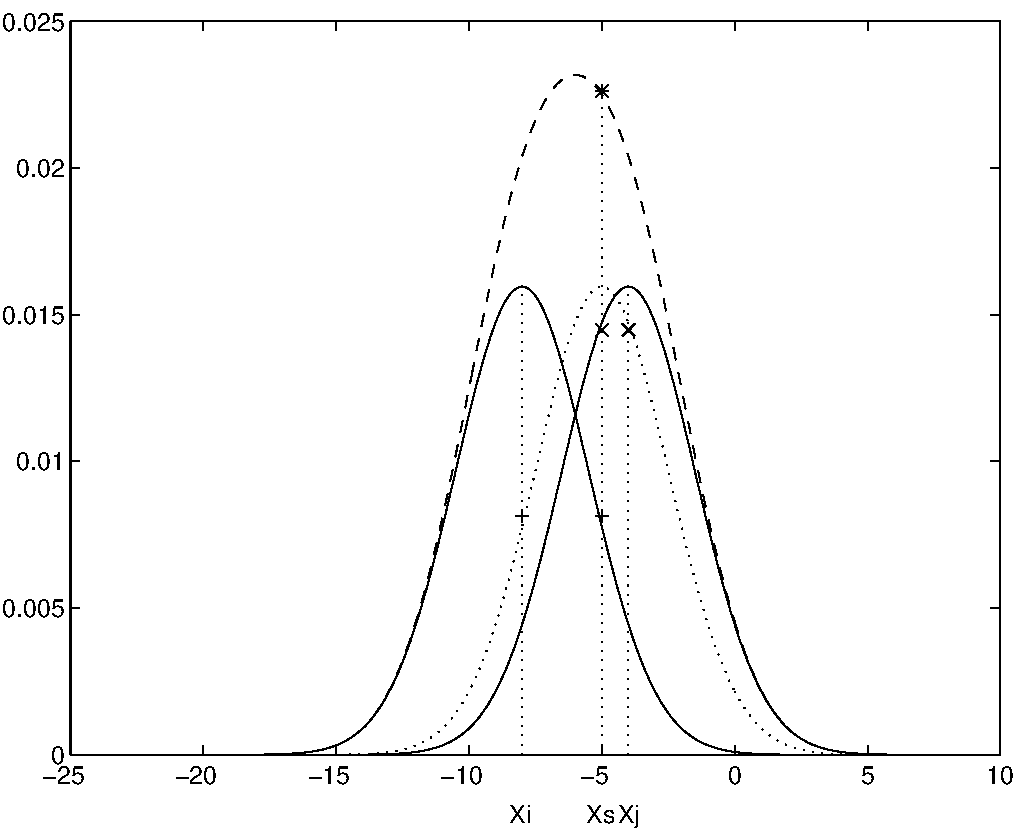
\includegraphics[width=0.6\textwidth]{figures/example.pdf}
    \caption{毕业论文的插图必须精心制作,线条要匀称,图面要整洁美观,插图应与正文呼应,不得与正文脱节。每幅插图应有图序和图题,全文插图可以统一编序,也可以逐章单独编序,不管采用哪种方式,图序必须连续,不得重复或跳缺。}
    \label{fig:1}
\end{figure}




\newpage
\section{结论}
本文开创性的提出了一种加入墨西哥辣椒版的番茄炒鸡蛋,它无缝衔接了淮扬菜和川菜两大菜系,提升了番茄炒蛋的味觉维度,进而弥合了上海和皖南人民对于番茄炒蛋的苛刻要求,实属一篇开创新的作品.当然,本文略有不足,有些人吃完拉肚子,有些人吃完说“好”的时候发生了下巴脱臼,还有一些人因为菜肴太好吃,偷偷没有吃完,把菜带回了家.但这些缺点都是小缺点,未来很容易就能补救,在我们开创性的研究下不值一提.




\newpage
\bibliography{references}



\newpage
\section*{致谢}
I would like to thank xxx for their advice.





\end{document}
